\chapter{Einleitung}
\section{NP-Vollst�ndigkeit}
Eine Sprache B ist \textbf{NP-Vollst\"andig} wenn gilt:
\begin{enumerate}
	\item $B \in NP$
	\item $\forall A \in NP: A \prec_p B$
\end{enumerate}

Notiz:\\
$A \prec_p B$ : $A$ ist polynomialzeitreduzierbar auf $B$

\section{Polynomialzeitreduktion}
Eine Sprache $A$ ist polynomialzeitreduzierbar auf Sprache $B$, $A \prec_p B$, wenn eine in polynomialer Zeit berechenbare Funktion $f:\Sigma*->\Sigma*$ existiert, f�r die gilt:\\
$\forall w:$
	$w \in A \iff f(w) \in B$

Die Funktion $f$ hei�t dann Polynomialzeitreduktion von $A$ nach $B$.

\section{Definition 3SAT}
Spezialform des Erf\"ullbarkeitsproblems
\begin{itemize}
	\item Symbol(literal):\\
	$x$ oder $\overline{x}$
	\item Klausel(clause):\\
	$(x_1 \lor \overline{x_2} \lor \overline{x_3} \lor x_4)$
	\item CNF-Formel(cnf-formula - conjunctive normal form):\\
	$(x_1 \lor \overline{x_2} \lor \overline{x_3} \lor x_4) \land (x_3 \lor \overline{x_5} \lor x_6) \land (x_3 \lor \overline{x_6})$
	\item 3CNF-Formel(3cnf-formula):\\
	$(x_1 \lor \overline{x_2} \lor \overline{x_3}) \land (x_3 \lor \overline{x_5} \lor x_6) \land (x_3 \lor \overline{x_6} \lor x_4) \land (x_4 \lor x_5 \lor x_6)$
\end{itemize}

$3SAT = \left\{ \right. \langle \phi \rangle | \phi$ ist eine erf�llbare 3CNF-Formel$\left. \right\}$

$\phi = 1 \iff \forall c_j$: mindestens ein Literal ist $true$ 

\chapter{Hamilton-Pfad-Problem}
\section{Definition}
\TODO{machen}

\section{Beweis}
\subsection{Gerichtet}
3SAT $\prec_p$ HAMPATH
\subsubsection{Darstellung $x_i$}
\begin{center}
	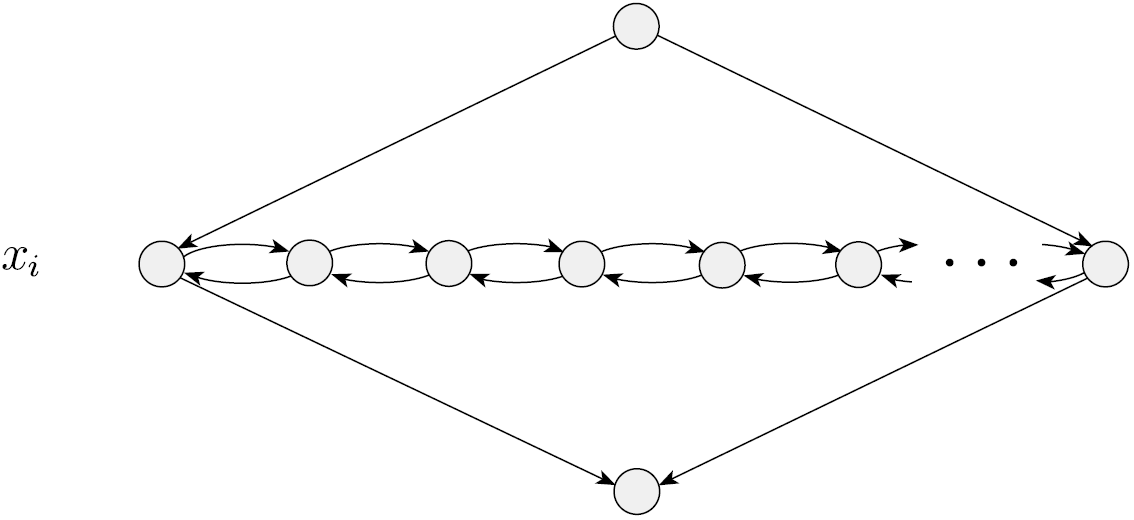
\includegraphics[width=14cm]{images/hampath/1}
\end{center}

\subsubsection{Darstellung $c_j$}
\begin{center}
	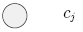
\includegraphics{images/hampath/2}
\end{center}

\subsubsection{High-level structure of G}
\begin{center}
	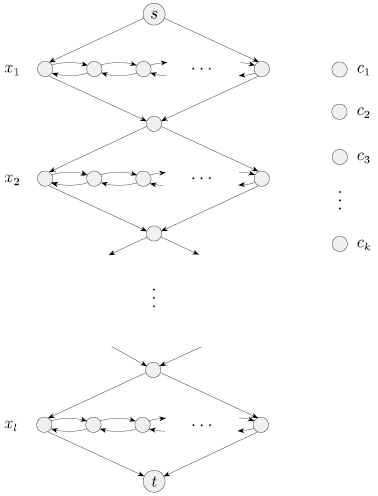
\includegraphics[width=14cm]{images/hampath/3}
\end{center}

\subsubsection{Horizontale Struktur im Diamond}
\begin{center}
	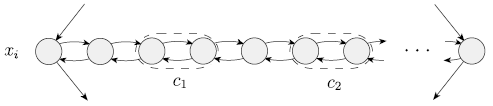
\includegraphics[width=14cm]{images/hampath/4}
\end{center}

\subsubsection{Zus\"atzliche Knoten wenn $x_i$ in $c_j$ ist}
\begin{center}
	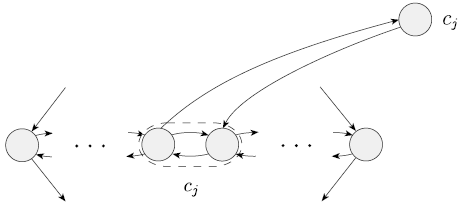
\includegraphics[width=14cm]{images/hampath/5}
\end{center}

\subsubsection{Zus\"atzliche Knoten wenn $\overline{x_i}$ in $c_j$ ist}
\begin{center}
	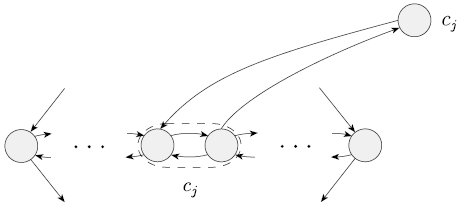
\includegraphics[width=14cm]{images/hampath/6}
\end{center}

\subsubsection{Zig-zagging and Zag-zigging}
\begin{center}
	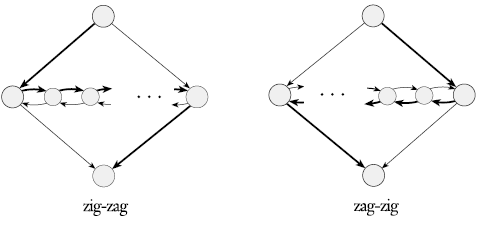
\includegraphics[width=14cm]{images/hampath/7}
\end{center}

\subsubsection{This situation cannot occur}
\begin{center}
	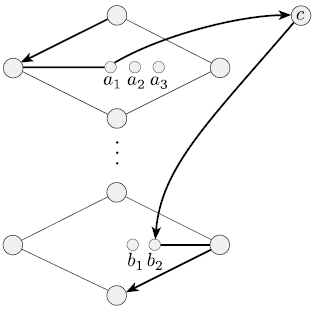
\includegraphics[width=14cm]{images/hampath/8}
\end{center}

\subsection{Ungerichtet}
\TODO{muss der auch rein?}

\chapter{SUBSET-SUM-Problem}
\section{Definition}
\TODO{machen}

\section{Beweis}
3SAT $\prec_p$ SUBSET-SUM